%!TeX root=../tese.tex
%("dica" para o editor de texto: este arquivo é parte de um documento maior)
% para saber mais: https://tex.stackexchange.com/q/78101

\chapter{Criação e validação dos protótipos da simulação}
\label{prototypes}

A partir dos requisitos listados no Capítulo \ref{design}, criamos dois protótipos iniciais de simulações desenvolvidos no Figma\footnote{\url{https://www.figma.com/}}, uma plataforma \textit{web} colaborativa para projetar interfaces. As Figuras~\ref{figure:brinquedos1} e~\ref{figure:festa1} mostram esses protótipos.

\begin{figure}[h!]
    \centering
    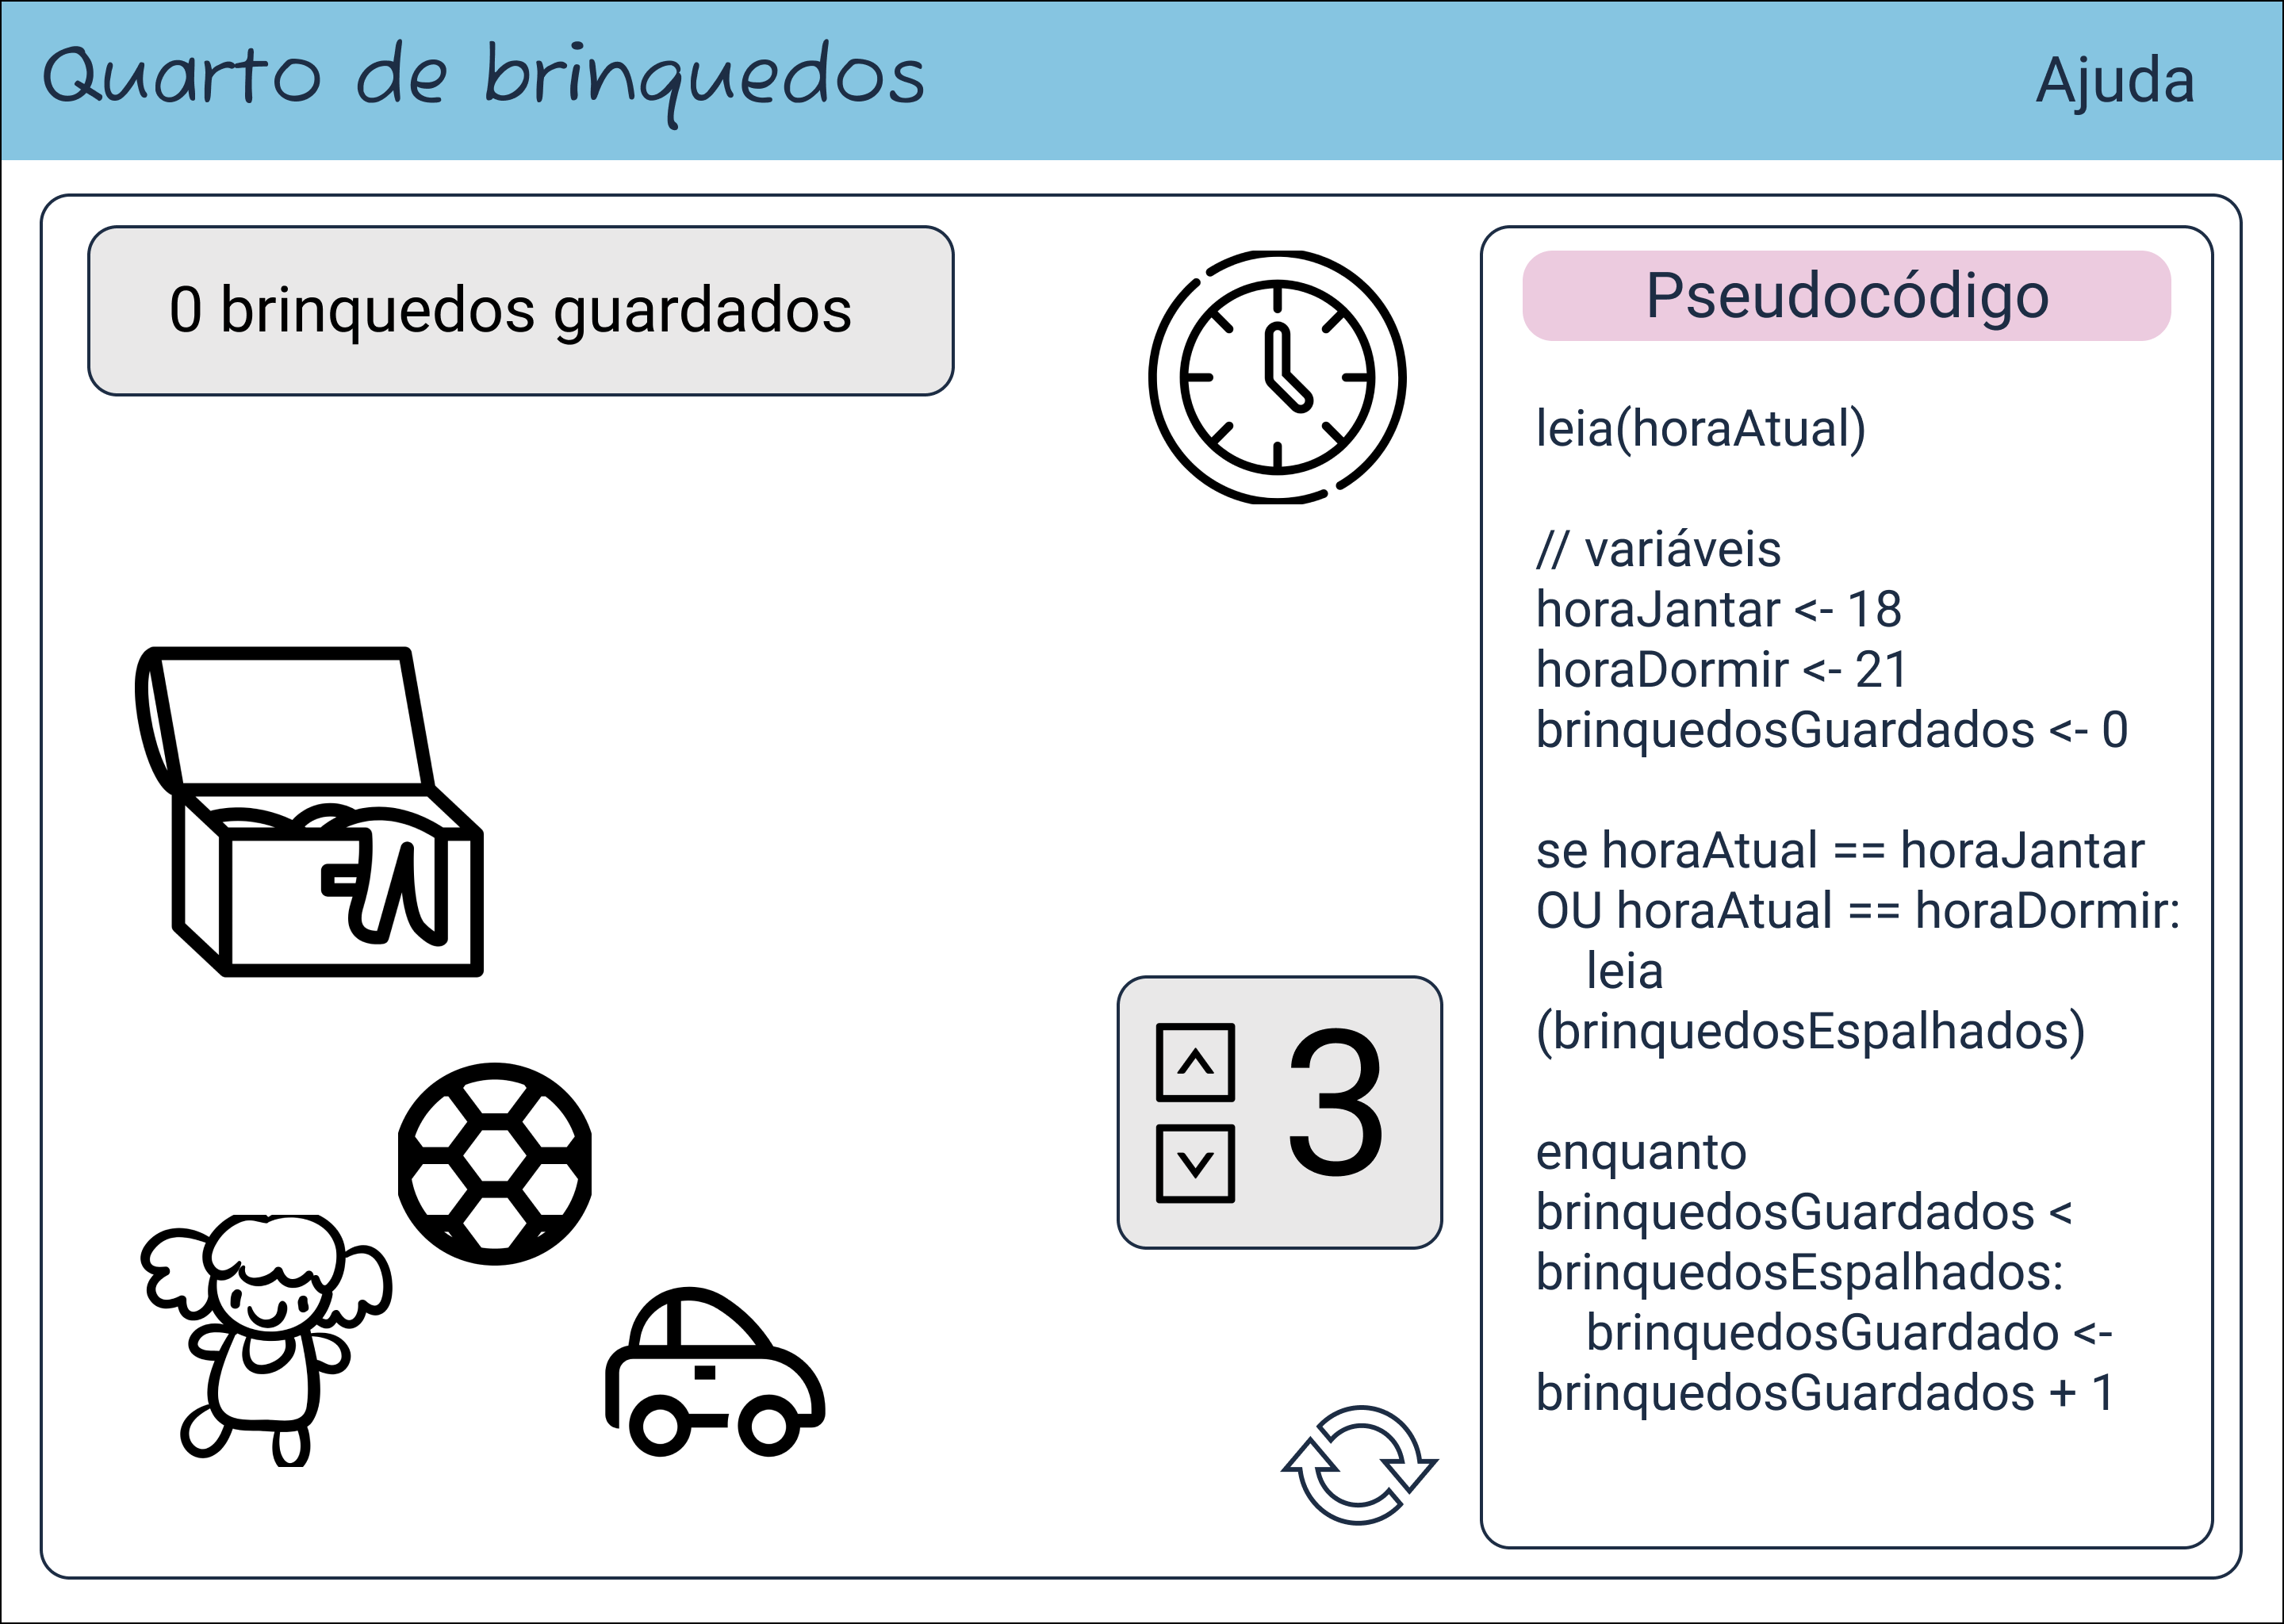
\includegraphics[scale=0.15]{prototipo_brinquedos1.png}
    \caption{Protótipo inicial da simulação \enquote{Quarto de Brinquedos}.}
    \label{figure:brinquedos1}
\end{figure}

Na Figura \ref{figure:brinquedos1}, temos um cenário de quarto de brinquedos. O protótipo da simulação apresenta elementos visuais como um relógio de parede, um baú para guardar objetos e brinquedos espalhados pelo chão. Além disso, temos dois painéis, um controle para regular a quantidade de brinquedos espalhados e um contador que mostra quantos brinquedos foram guardados. Ainda, o protótipo apresenta um pseudocódigo associado à simulação.

A princípio, a ideia dessa simulação é apresentar duas interações possíveis: alterar a hora no relógio e guardar os brinquedos no baú de forma iterativa. Com isso, queremos abordar o conceito de variáveis, principalmente, com a ação de guardar os objetos em um contêiner; de entrada, com a informação recebida através da interação com o usuário ao alterar o horário; de operadores, na comparação de expressões simples e complexas com conectivos lógicos, e na operação de adição contida na ação de guardar os brinquedos; de condicionais, verificando se é o momento de organizar o quarto; e de laços de repetição, repetindo a ação de guardar cada objeto até que o quarto esteja organizado.

\begin{figure}[h!]
    \centering
    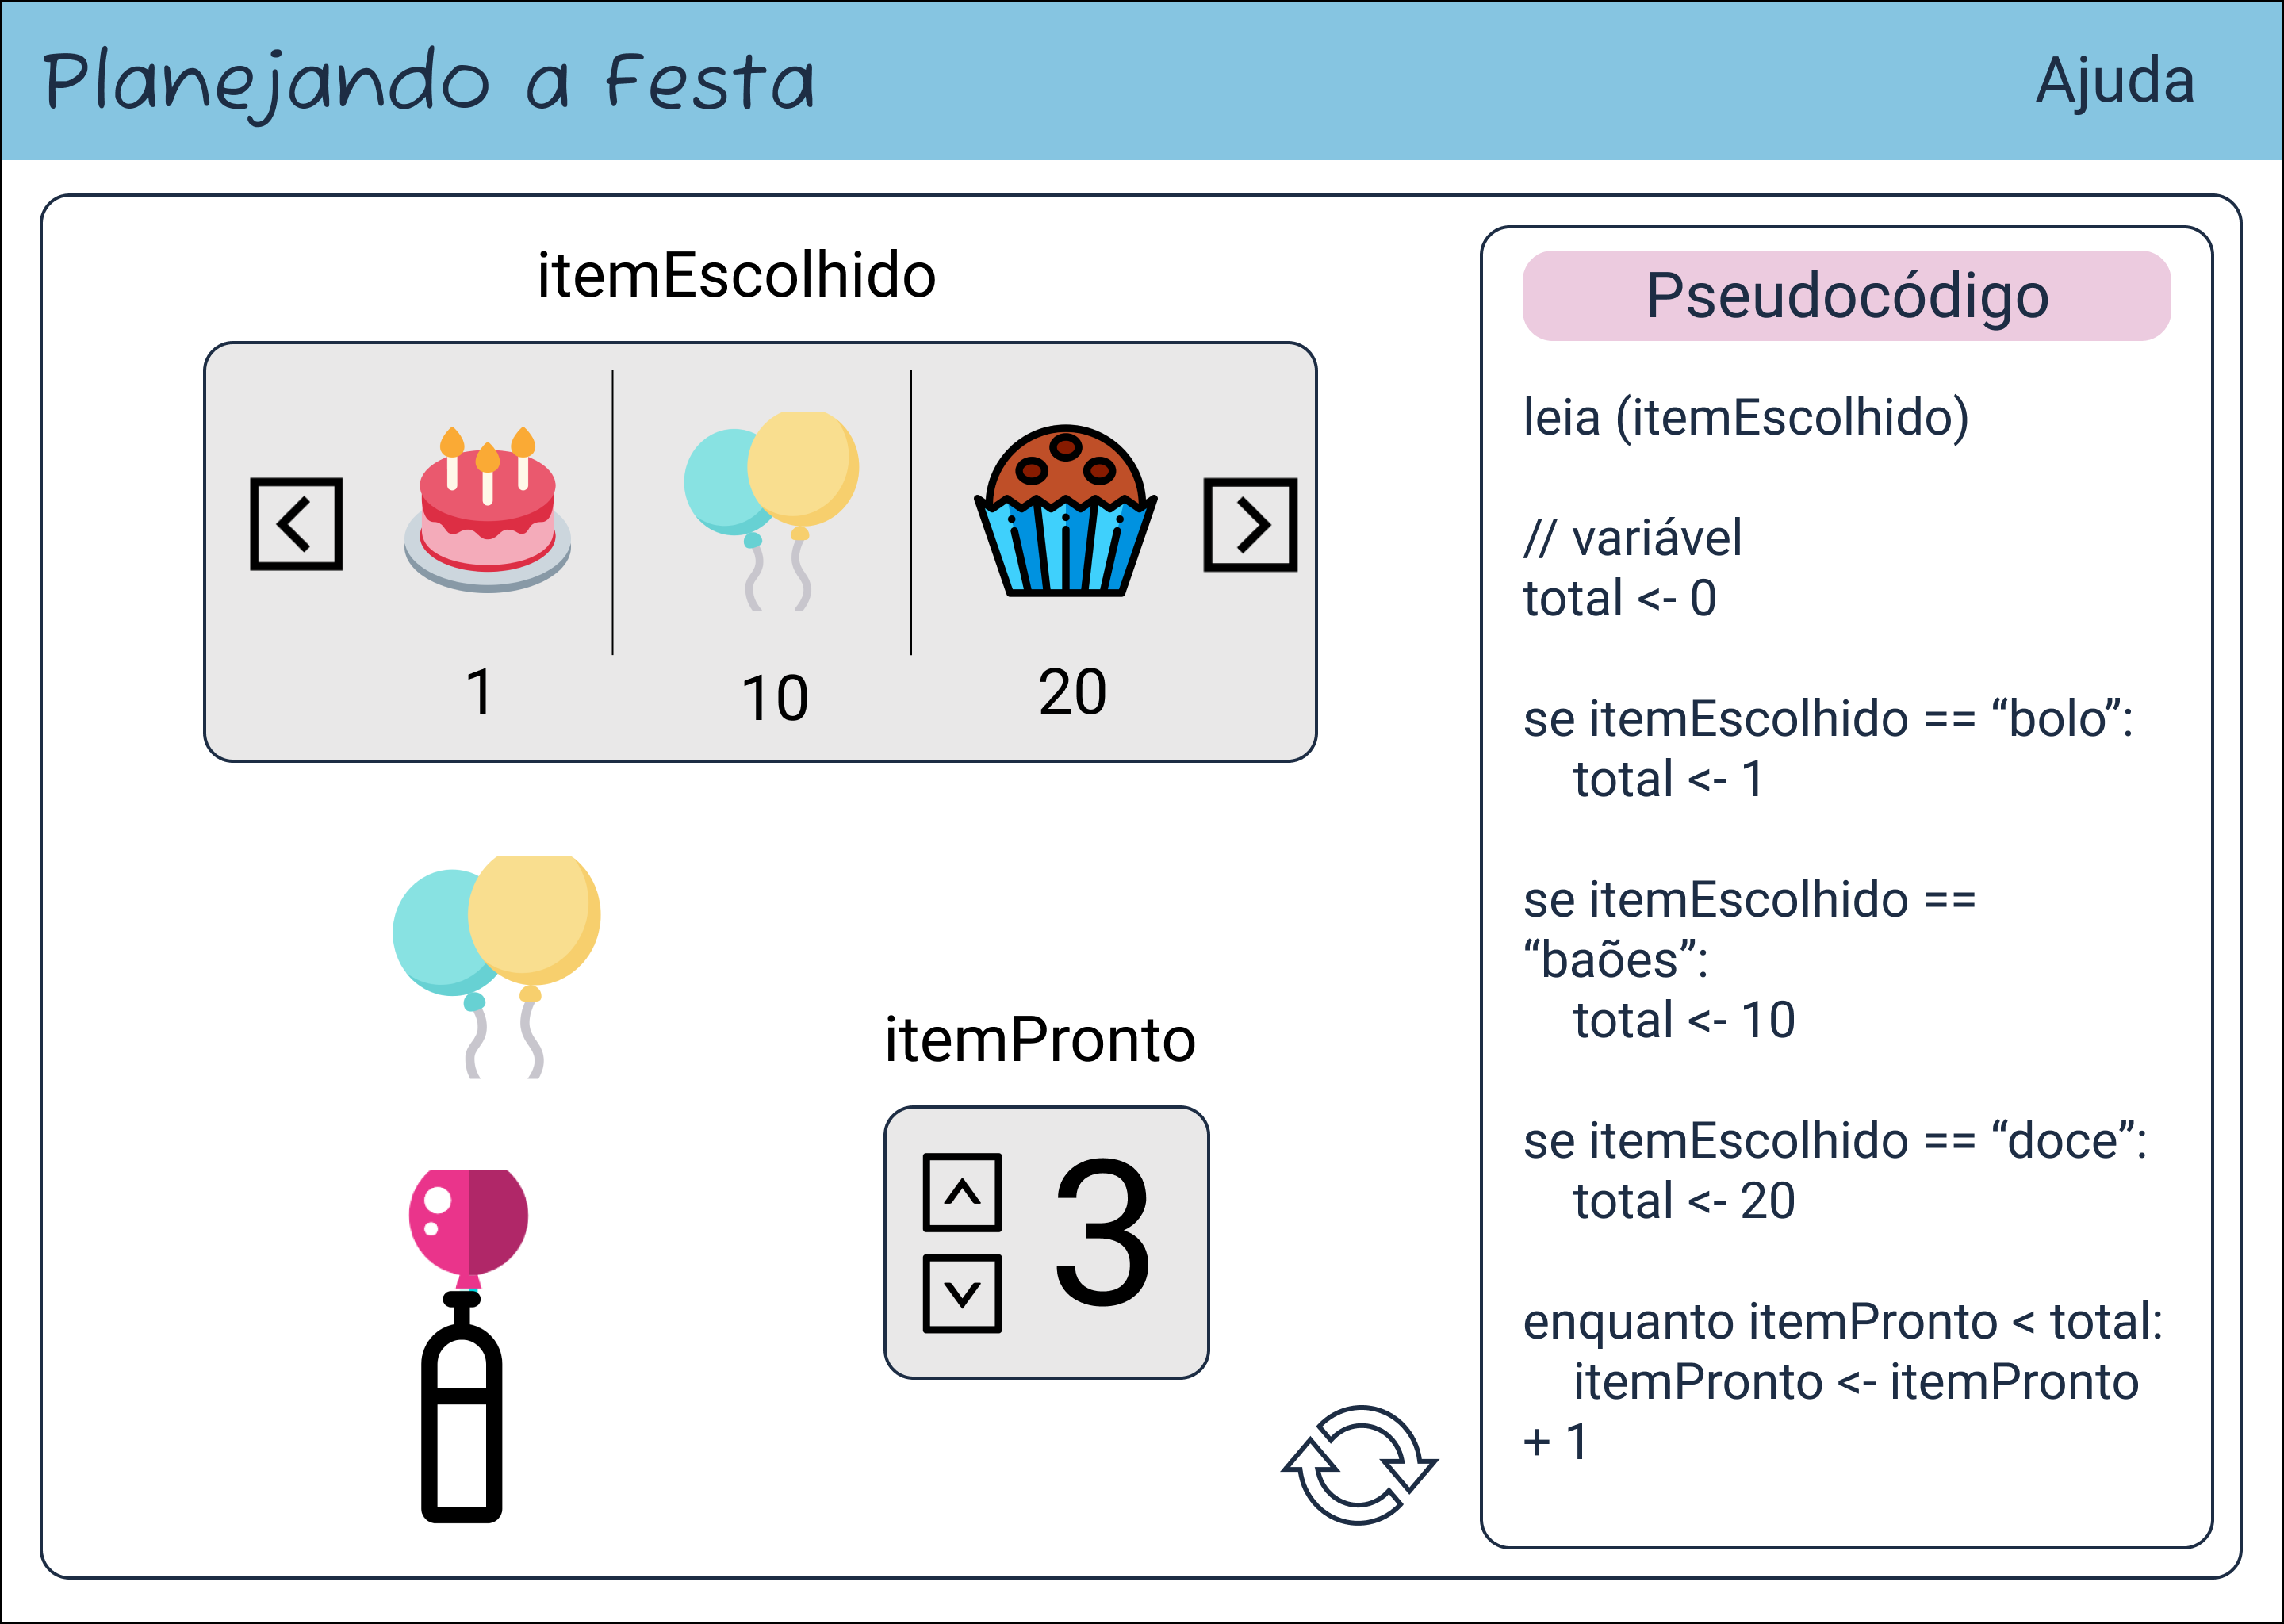
\includegraphics[scale=0.15]{prototipo_festa1.png}
    \caption{Protótipo inicial da simulação \enquote{Planejando a Festa}.}
    \label{figure:festa1}
\end{figure}

A Figura \ref{figure:festa1} apresenta um cenário de planejamento de uma festa. Nele há elementos visuais que representam itens que podem ser escolhidos para incorporar uma festa de aniversário. Ademais, temos um contador que mostra quantos itens referentes ao escolhido já estão preparados. Nessa simulação, o usuário pode ter duas interações: escolher um item para a festa e \enquote{prepará-lo} (incrementar um determinado item) até estar completo. Deste modo, nesse cenário, abordamos os conceitos de variáveis, por meio do total de objetos que devemos ter de acordo com a escolha do item; de entrada, a partir da escolha de um item para a festa; de operadores, na comparação de expressões simples, e na operação de adição contida na ação de preparar um item; de condicionais, verificando qual item foi escolhido; e de laços de repetição, conforme incremento dos objetos até atingirem o total de acordo com cada elemento.

Com os protótipos iniciais projetados, foram realizadas algumas mudanças antes de apresentá-los, conforme sugestões da professora Kelly Braghetto. As Figuras \ref{figure:brinquedos2} e \ref{figure:festa2} mostram as alterações sugeridas para os artefatos.

\begin{figure}[h!]
    \centering
    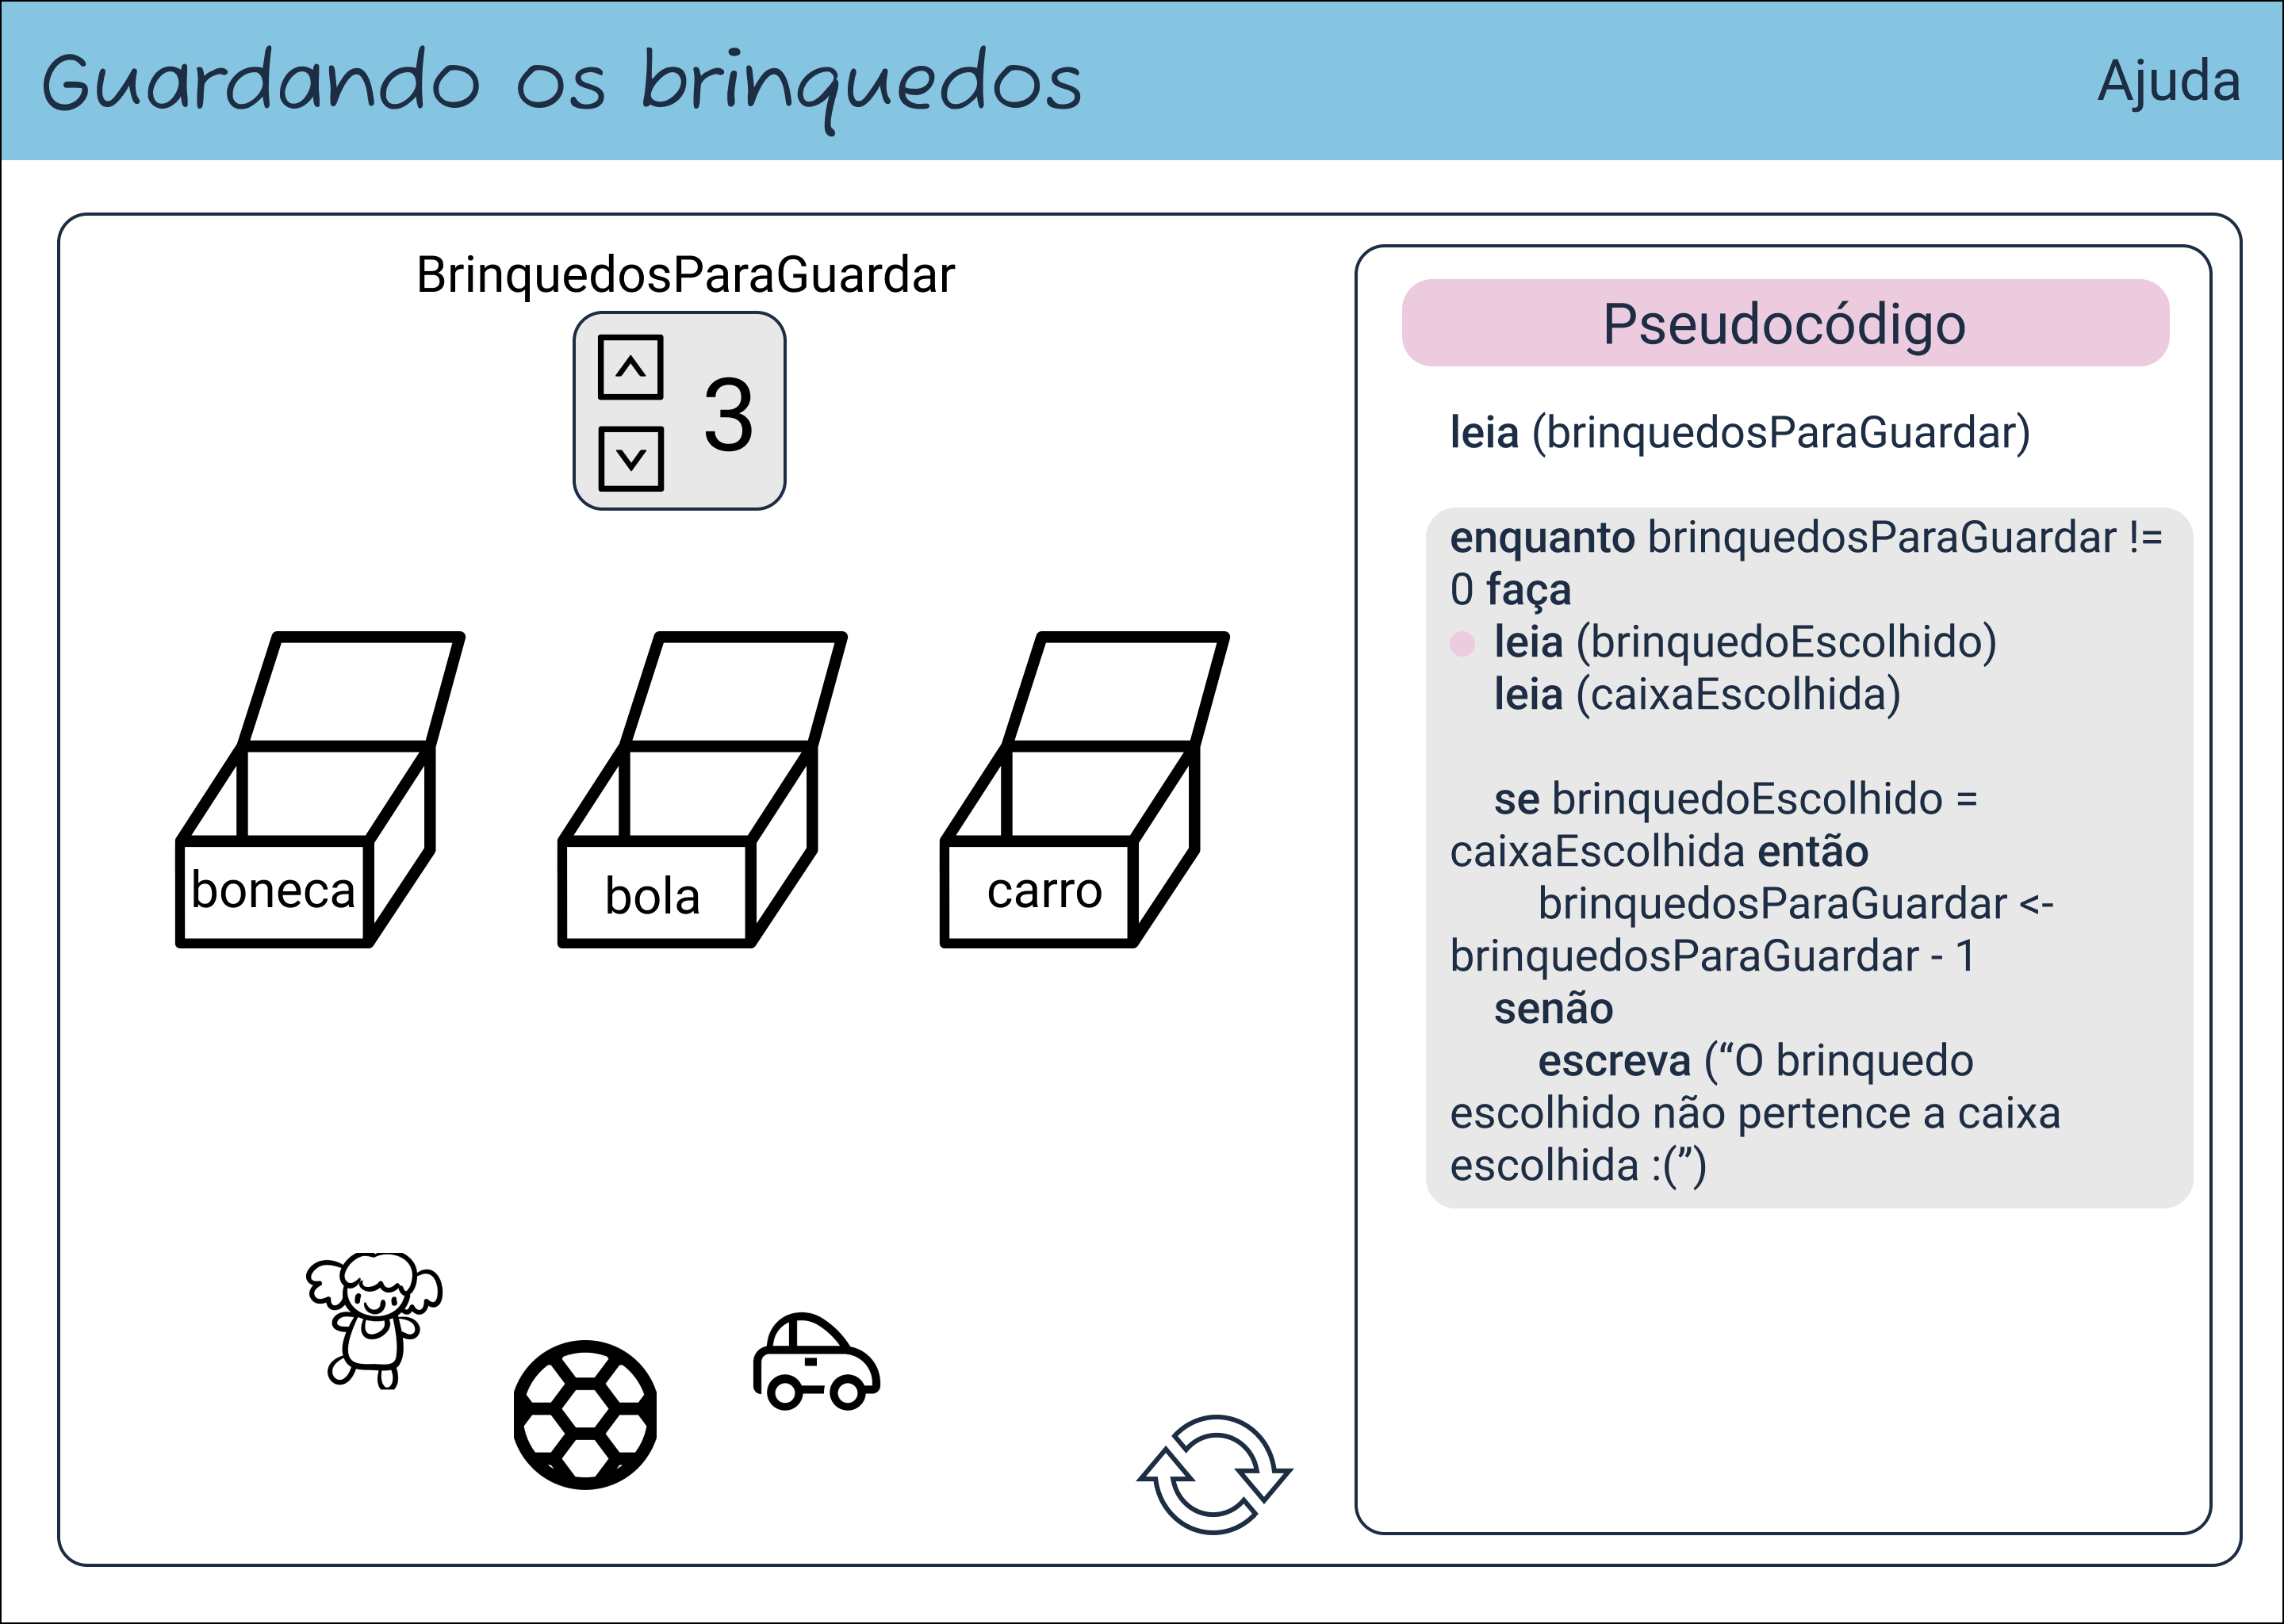
\includegraphics[scale=0.15]{prototipo_brinquedos2.png}
    \caption{Protótipo da simulação \enquote{Guardando os Brinquedos} após validação.}
    \label{figure:brinquedos2}
\end{figure}

\begin{figure}[h!]
    \centering
    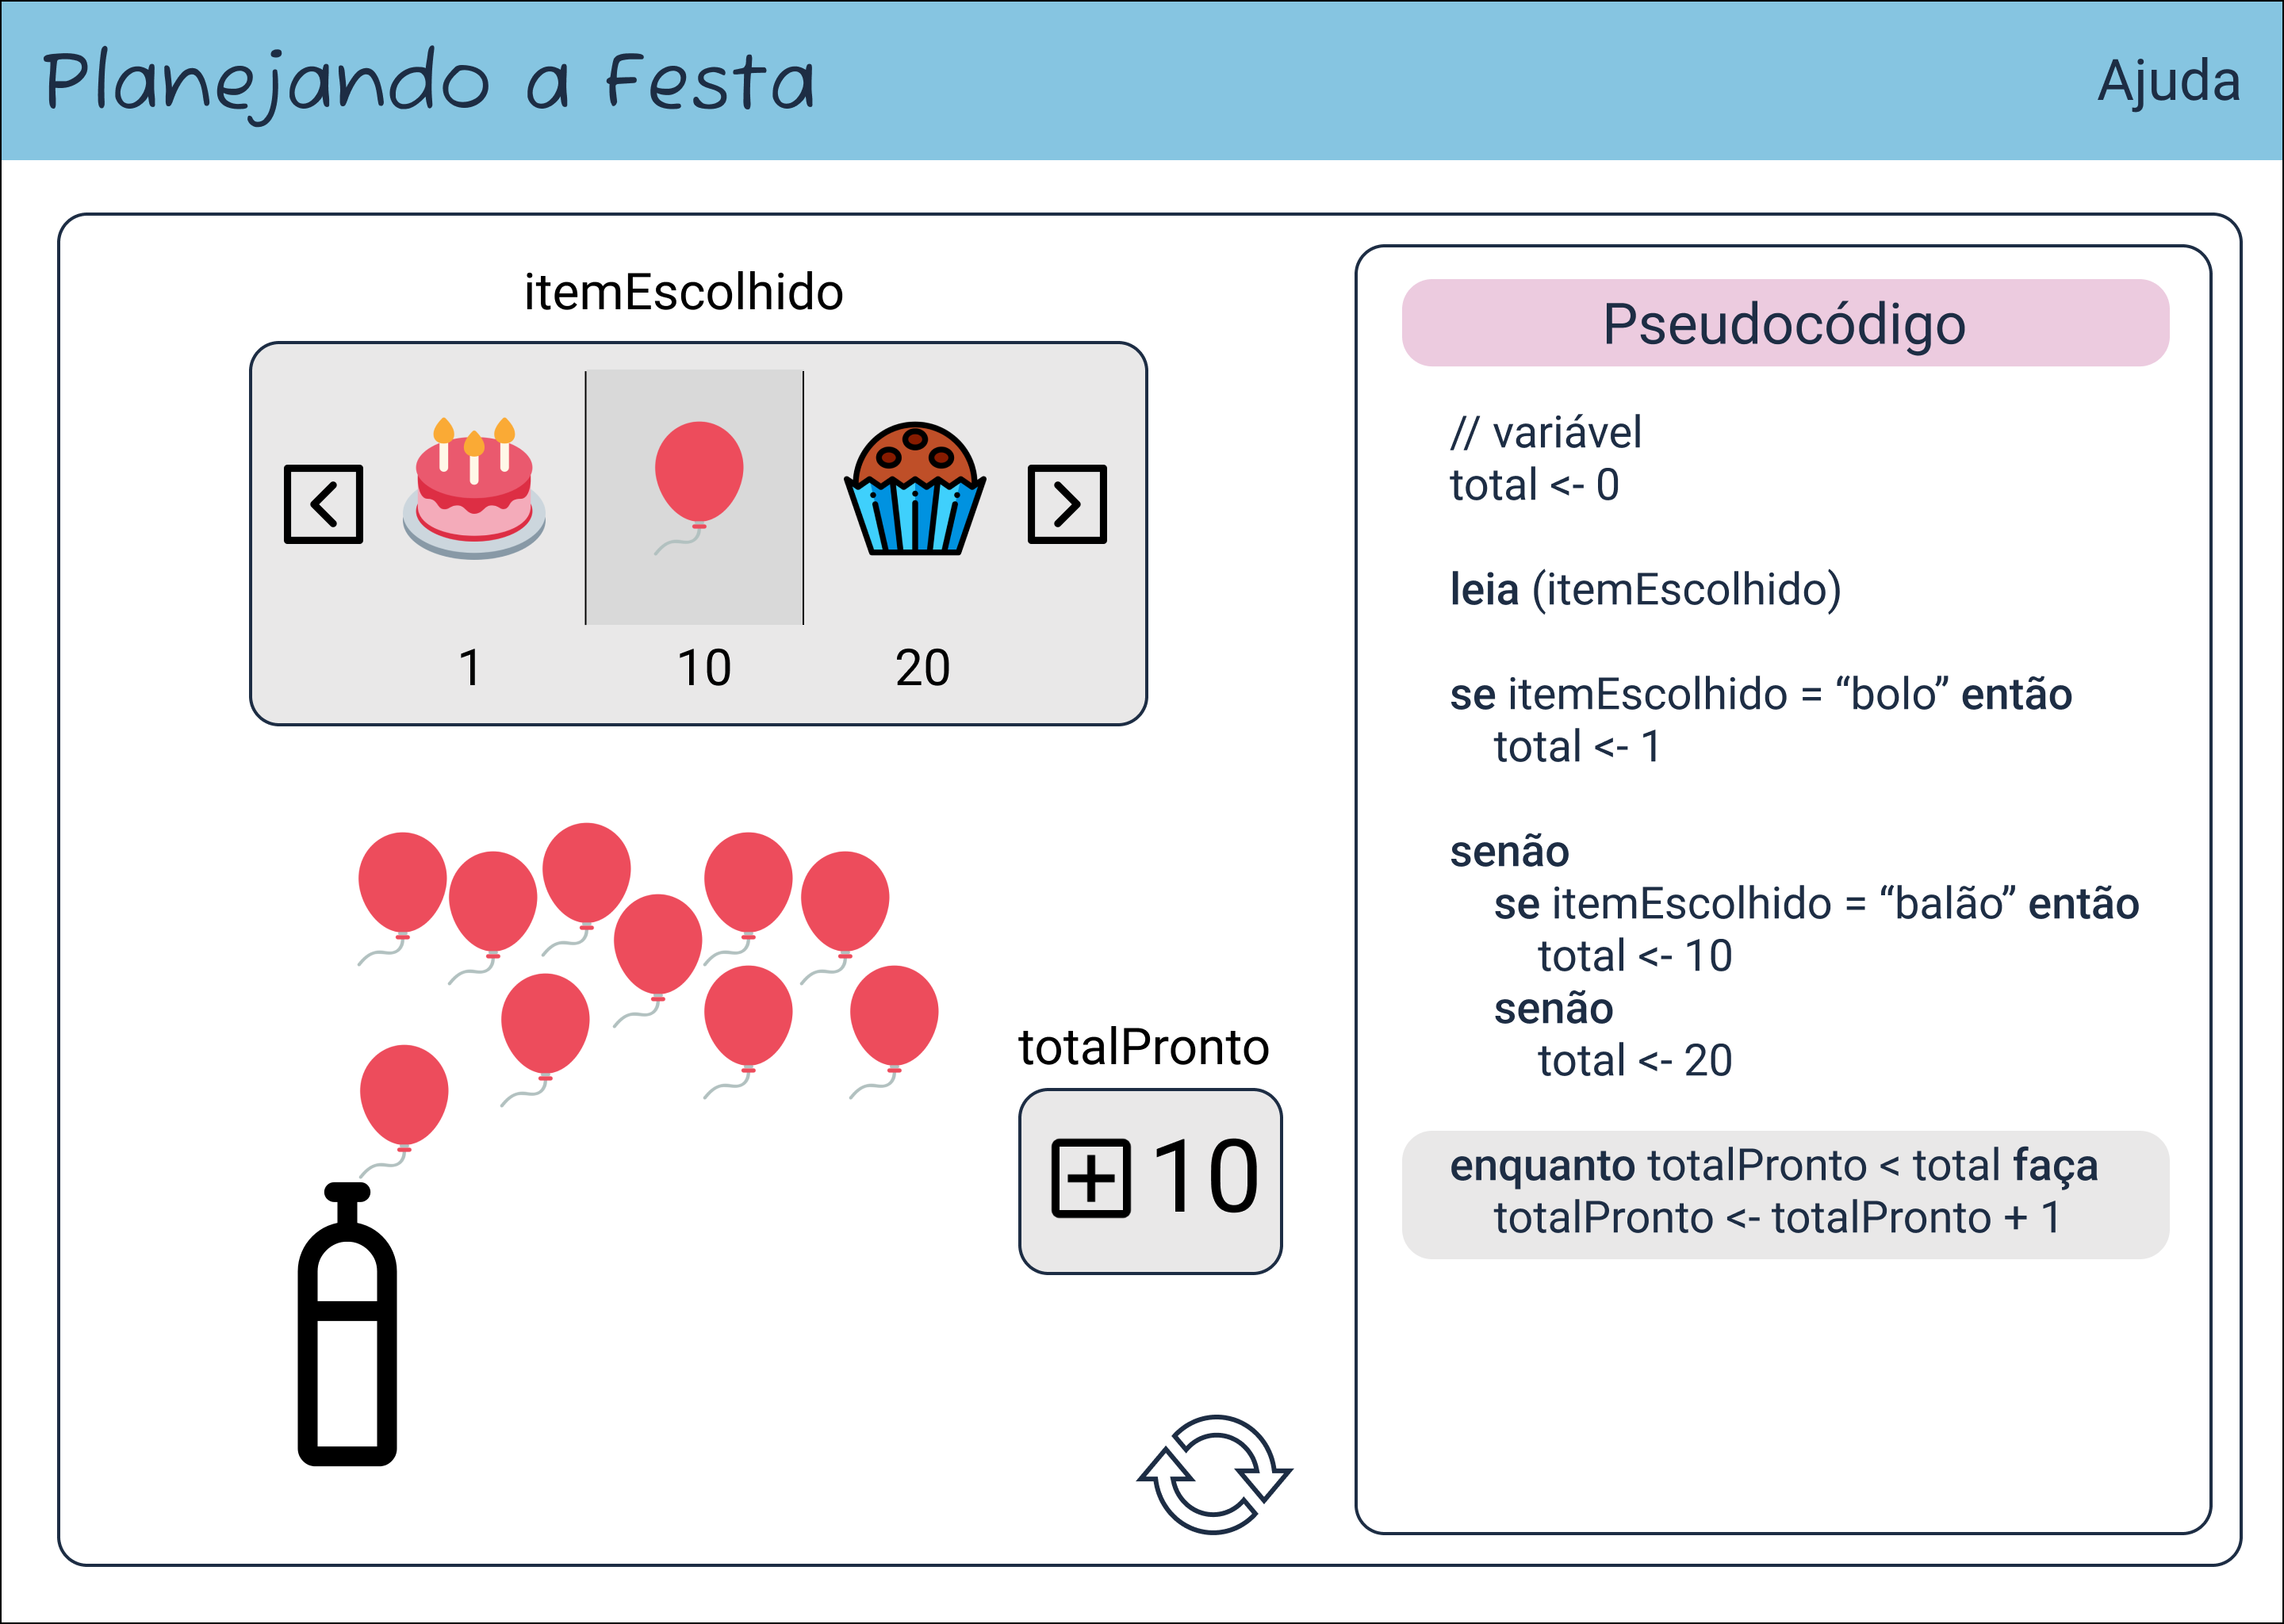
\includegraphics[scale=0.15]{prototipo_festa2.png}
    \caption{Protótipo da simulação \enquote{Planejando a Festa} após validação.}
    \label{figure:festa2}
\end{figure}

Na Figura \ref{figure:brinquedos2} podemos observar a nova simulação \enquote{Guardando os Brinquedos}, que teve sua lógica modificada para simplificar as interações com os elementos visuais e melhorar a usabilidade. Nele, há um contador que permite selecionar até três brinquedos para guardar em suas respectivas caixas. As interações possíveis nessa simulação são: incrementar o contador para escolher quantos brinquedos guardar e, após esta escolha, escolher brinquedo e caixa correspondente. A cada brinquedo guardado corretamente, o valor do contador deve ser subtraído de um. Nesse cenário, abordamos os conceitos de variáveis, na quantidade de brinquedos para guardar e nos itens (brinquedo e caixa) escolhidos; de entrada e saída, na leituras das variáveis e na escrita da mensagem quando o brinquedo e a caixa escolhida não correspondem; de operadores, na comparação de expressões simples e na operação de subtração contida na ação de guardar os brinquedos; de condicionais, verificando se o brinquedo e a caixa escolhida correspondem; e de laços de repetição, repetindo a ação de guardar cada objeto até não sobrar mais nenhum.

Já na nova versão da simulação \enquote{Planejando a Festa} (Figura \ref{figure:festa2}), podemos observar a mudança no controle do incremento do contador que indica a quantidade de itens totais prontos. Além disso, no geral, as sugestões implementadas nos protótipos envolveram a melhoria nos nomes das variáveis, a incorporação do conceito de saída e o destaque na parte do pseudocódigo em que está ocorrendo a interação na simulação.

Em seguida, em conversas com os avaliadores, foi possível obter \textit{feedbacks} para verificar a usabilidade e utilidade do MVP a partir dos protótipos projetados, possibilitando o refinamento deles e a escolha de um artefato para implementação. A simulação \enquote{Planejando a Festa} se mostrou mais interessante e com maiores possibilidades de interações e, por isso, foi escolhida como artefato a ser implementado. Ademais, o público alvo definido para a aplicação do MVP foram crianças no Ensino Fundamental II, a partir do 6° ano.

As demais sugestões recebidas pelos avaliadores levaram em conta, portanto, o protótipo escolhido e foram aplicadas diretamente na implementação do artefato. Dessa forma, a lógica da simulação \enquote{Planejando a Festa} foi alterada para melhorar a sua usabilidade e as interações com os elementos visuais. No Capítulo~\ref{cap_mvp}, descrevemos os detalhes da implementação com as modificações realizadas.
